% MA211 - Lecture 19
\documentclass[pdftex, xcolor=pdftex, dvipsnames,handout]{beamer}

\usetheme{MA211}
\usepackage{thumbpdf}
\usepackage{wasysym}
%\usepackage{ucs}
\usepackage[utf8]{inputenc}
\usepackage{pgf,pgfarrows,pgfnodes,pgfautomata,pgfheaps,pgfshade}
\usepackage{verbatim}

\usepackage{eurosym}
\usepackage{euler}

\usepackage{calc}               % Simple computations with LaTeX variables
%\usepackage[hang]{caption2}     % Improved captions

\usepackage{graphicx}           % Standard graphics package

\usepackage{amsmath, amsthm, amssymb}


\newcommand{\fquad}{\mbox{\qquad}}
\newcommand{\bull}{$\bullet$ }

\newcommand {\I} {\mathcal I}
\newcommand {\calI} {\mathcal I}
\def\disint{\displaystyle\int}

\DeclareMathOperator{\D}{d}
\newcommand{\dydx}{\frac{\D y}{\D x}}

%\definecolor{gray}{rgb}{0.69, 0.69, 0.69} \newcommand{\gray}[1]{\textcolor{gray}{#1}}
\definecolor{dogreen}{rgb}{0.33, 0.42, 0.18} \newcommand{\dogreen}[1]{\textcolor{dogreen}{#1}}
\definecolor{maroon}{rgb}{.5,0.2,0.2}\newcommand{\maroon}[1]{\textcolor{maroon}{#1}}
\definecolor{greena}{rgb}{.1,0.581,0.1}\newcommand{\greena}[1]{\textcolor{greena}{#1}}

\definecolor{blue4}{rgb}{0,0,.545}
\newcommand{\Blue}[1]{\textcolor{blue}{#1}}
\newcommand{\Red}[1]{\textcolor{red}{#1}}
\definecolor{pink}{rgb}{1.,0.75,0.8}
\definecolor{darkred}{rgb}{0.5,0.0,0.0}
\definecolor{darkgreen}{rgb}{0,0.3,0.3}
\definecolor{purple}{rgb}{0,0.3,0.3}
\definecolor{darkblue}{rgb}{0.0, 0.0, .5}
\definecolor{dpurple}{rgb}{.3,.0,.3}
\newcommand{\Green}[1]{\textcolor{darkgreen}{#1}}
\newcommand{\DRed}[1]{\textcolor{darkred}{#1}}
\newcommand{\DBlue}[1]{\textcolor{darkblue}{#1}}
\newcommand{\Purple}[1]{\textcolor{dpurple}{#1}}
\newcommand{\Emph}[1]{\textcolor{darkred}{\textbf{\it #1}}}
\newcommand{\remph}[1]{\textcolor{darkred}{\textbf{\emph{#1}}}}
\newcommand{\bemph}[1]{\textcolor{darkblue}{\textbf{\emph{#1}}}}
\newcommand{\gemph}[1]{\textcolor{darkgreen}{\textbf{\emph{#1}}}}
\newcommand{\Bf}[1]{\textcolor{darkblue}{\textbf{#1}}}
\newcommand{\Gf}[1]{\textcolor{darkgreen}{\textbf{#1}}}
\newcommand{\Rf}[1]{\textcolor{red}{\textbf{#1}}}
\newcommand{\Rmf}[1]{\textcolor{red}{\mathbf{#1}}}

\newcommand{\Conj}[1]{\overline{#1}}

\newcommand{\code}[1]{\textcolor{darkblue}{\texttt{\textbf{#1}}}}
\newcommand{\icode}[1]{{\blue\texttt{\textbf{\emph{#1}}}}}
\newcommand{\gcode}[1]{{\Green{\texttt{\textbf{\emph{#1}}}}}}
\newcommand{\out}[1]{\texttt{\emph{\textbf{\Green{#1}}}}}





\newenvironment{vminipage}%
{\begin{Sbox}\begin{minipage}\begin{small}\begin{verbatim}}%
{\end{verbatim}\end{small}\end{minipage}\end{Sbox}\fbox{\TheSbox}}

\newenvironment{nminipage}%
{\begin{Sbox}\begin{minipage}}%
{\end{minipage}\end{Sbox}\fbox{\TheSbox}}


\let\Arg\relax\DeclareMathOperator{\Arg}{\mathtt{Arg}}
\let\Arg\relax\DeclareMathOperator{\e}{\mathtt{e}}

\newcommand {\AND} {\wedge}
\newcommand {\OR} {\vee}
\newcommand {\NOT} {\neg}
\newcommand {\IMPLIES} {\rightarrow}
%\newcommand {\IFF} {\leftrightarrow}
\renewcommand {\iff} {\Leftrightarrow}
\newcommand {\NAND} {\uparrow}
\newcommand {\NOR} {\downarrow}
\newcommand {\XOR} {\otimes}

\newenvironment{citemize}% Colour items
{\begin{description}}%
{\end{description}}

\newcommand {\maroonitem}{\item[\maroon{$\bullet$}]}

\newcommand {\gitem} {\item {\includegraphics[width=.4cm,angle=-10]{img/green-bullet-on-white.ps}}}
\newcommand {\ritem} {\item {\includegraphics[width=.4cm,angle=-10]{img/red-bullet-on-white.ps}}}
\newcommand {\yitem} {\item {\includegraphics[width=.4cm,angle=-10]{img/yellow-bullet-on-white.ps}}}
\newcommand {\bitem} {\item {\includegraphics[width=.4cm,angle=-10]{img/blue-bullet-on-white.ps}}}

\newcommand {\greenitem} {\item {\includegraphics[width=.4cm,angle=-10]{img/green-bullet-on-white.ps}}}
\newcommand {\reditem} {\item {\includegraphics[width=.4cm,angle=-10]{img/red-bullet-on-white.ps}}}
\newcommand {\yellowitem} {\item {\includegraphics[width=.4cm,angle=-10]{img/yellow-bullet-on-white.ps}}}
\newcommand {\blueitem} {\item {\includegraphics[width=.4cm,angle=-10]{img/blue-bullet-on-white.ps}}}

\newcommand {\eq}[1]%
  {$\DBlue{#1}$}
\newcommand {\eqd}[1]%
  {$\displaystyle\DBlue{#1}$}
%\newcommand{\eq}[1]{\boldmath \DBlue{$#1$}}


\newcommand {\csf}{\centerslidesfalse}
\newcommand {\cst}{\centerslidestrue}

\newcommand {\vecii}[2] {   \big(\begin{smallmatrix} #1 \\ #2 \end{smallmatrix}\big)}
\newcommand{\atwo}[2]{\left(\!\!\begin{array}{c} #1 \\ #2 \end{array}\!\!\right)}


\newcommand{\C}{\mathbb{C}}
\newcommand{\Q}{\mathbb{Q}}
\newcommand{\R}{\mathbb{R}}
\newcommand{\N}{\mathbb{N}}
\newcommand{\Z}{\protect\mathbb{Z}}  % protect for index.
\newcommand {\Rs}{ \mathbb{R}}
\newcommand {\Cs}{ \mathbb{C}}
\newcommand {\Rnn}{ \mathbb{R}^{n \times n}}
\newcommand {\Rn}{ \mathbb{R}^{n}}


\newcommand{\mblock}{%
\setbeamercolor*{block title}{bg=maroon,fg=white}
\setbeamercolor*{block body}{bg=white,fg=maroon}
}%

\newcommand{\bblock}{%
\setbeamercolor*{block title}{bg=Steel,fg=white}
\setbeamercolor*{block body}{bg=Mylightgray,fg=Steel}
}%

\newcommand{\gblock}{%
\setbeamercolor*{block title}{bg=Green,fg=white}
\setbeamercolor*{block body}{bg=Mylightgray,fg=darkgreen}
}%


\newcommand{\rblock}{%
\setbeamercolor*{block title}{bg=Red,fg=white}
\setbeamercolor*{block body}{bg=white,fg=Black}
}%


\newcommand{\TakeNotes}{
\includegraphics[width=2cm]{TakeNote}}

\def\eps{\varepsilon}
\newcommand {\del}[2]{ {\frac{\partial #1}{\partial #2}}}
\newcommand {\x}[1]{x^{[#1]}}
\newcommand {\delx}{ {\frac{\partial}{\partial x}}}
\newcommand {\delt}{ {\frac{\partial}{\partial t}}}
\newcommand {\dely}{ {\frac{\partial}{\partial y}}}
\newcommand {\ith}{{(i)}}
\renewcommand {\vec}[1]{ {\boldsymbol{#1}}}
\newcommand {\Oh} {\mathcal O}
\newcommand {\Err} {\mathcal E}
%\newcommand {\th} {\mathrm{th}}
\DeclareMathOperator{\fl}{fl}
\DeclareMathOperator{\sign}{sign}
\DeclareMathOperator{\Cond}{Cond} 
\DeclareMathOperator{\cond}{cond}
\DeclareMathOperator{\diag}{diag} 
\DeclareMathOperator{\sym}{sym} 
\DeclareMathOperator{\Trace}{Trace}
%\DeclareMathOperator{\D}{d}
\DeclareMathOperator{\E}{e}

\newcommand {\Rsym}{{ \mathbb{R}^{n \times n}_\mathrm{sym}}}

\newcommand {\st} {\mathrm{st}}
\newcommand {\nd} {\mathrm{nd}}


\parskip .25cm


\theoremstyle{definition}
\newtheorem{exercise}{Exercise}[section]
\newtheorem{method}{Method}[section]

\newcommand{\Header}[1]{\begin{center}{\Large \Bf{#1}}\end{center}}

\subtitle{MA211}
\title{Lecture 19: Improper Integrals -Type 1}

\author{Dr Niall Madden}

\date{\Large Wed $12^\mathrm{th}$ Nov 2008}


\begin{document}

\setcounter{framenumber}{-1}
\frame{

%\begin{columns}[c]
%\column{0.45\textwidth}
%\centering
%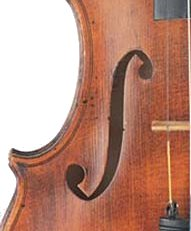
\includegraphics[width=4cm]{images/violin}
%
%
%\column{0.55\textwidth}
\begin{block}{}
\begin{center}
\begin{large}
 \insertsubtitle
\end{large}

\vspace{.1cm}

\begin{Large}
\textbf{\inserttitle}
\end{Large}


\vspace{.3cm}

{\insertdate}

\end{center}
\end{block}

\begin{center}
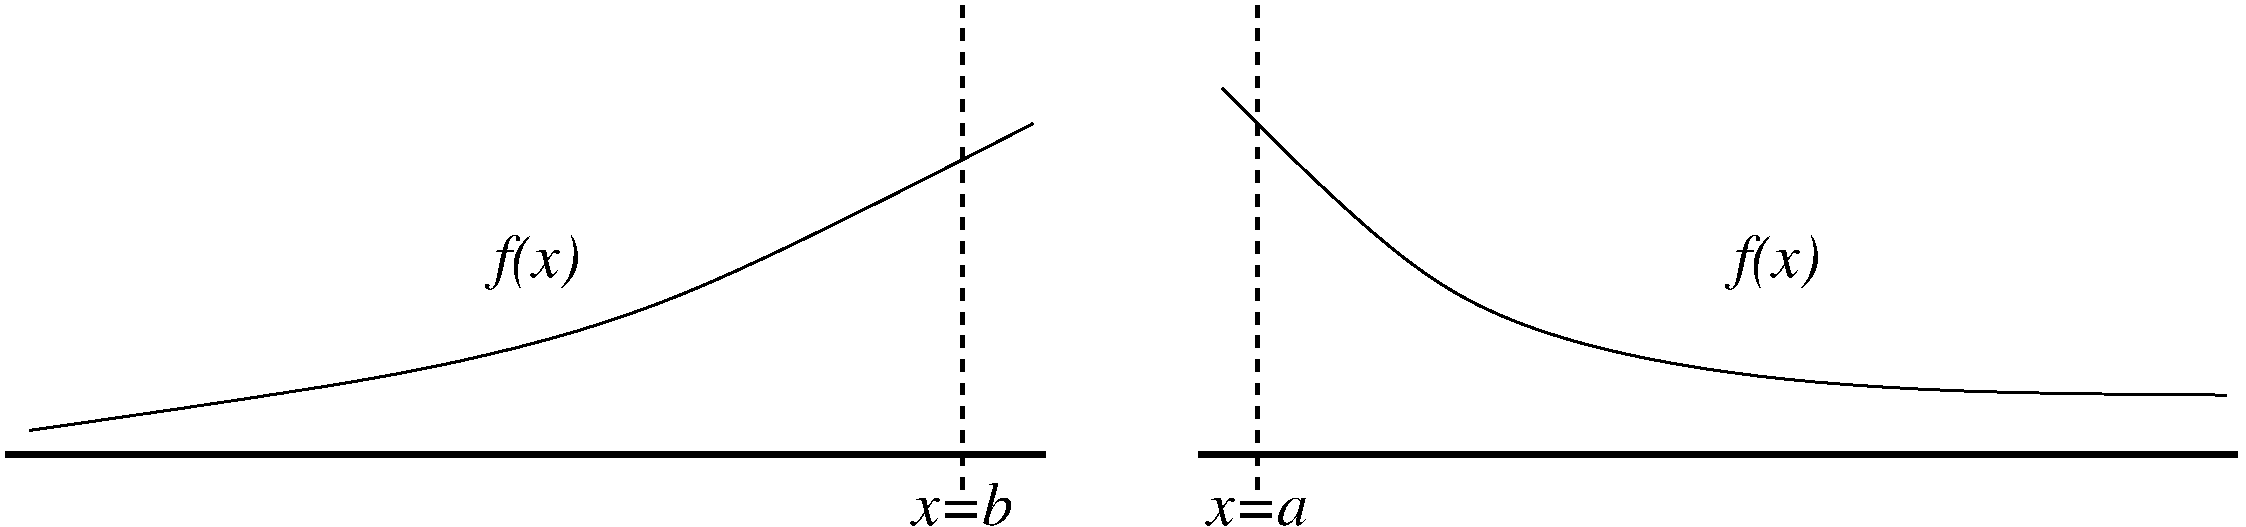
\includegraphics[width=8cm]{images/Improper1}
%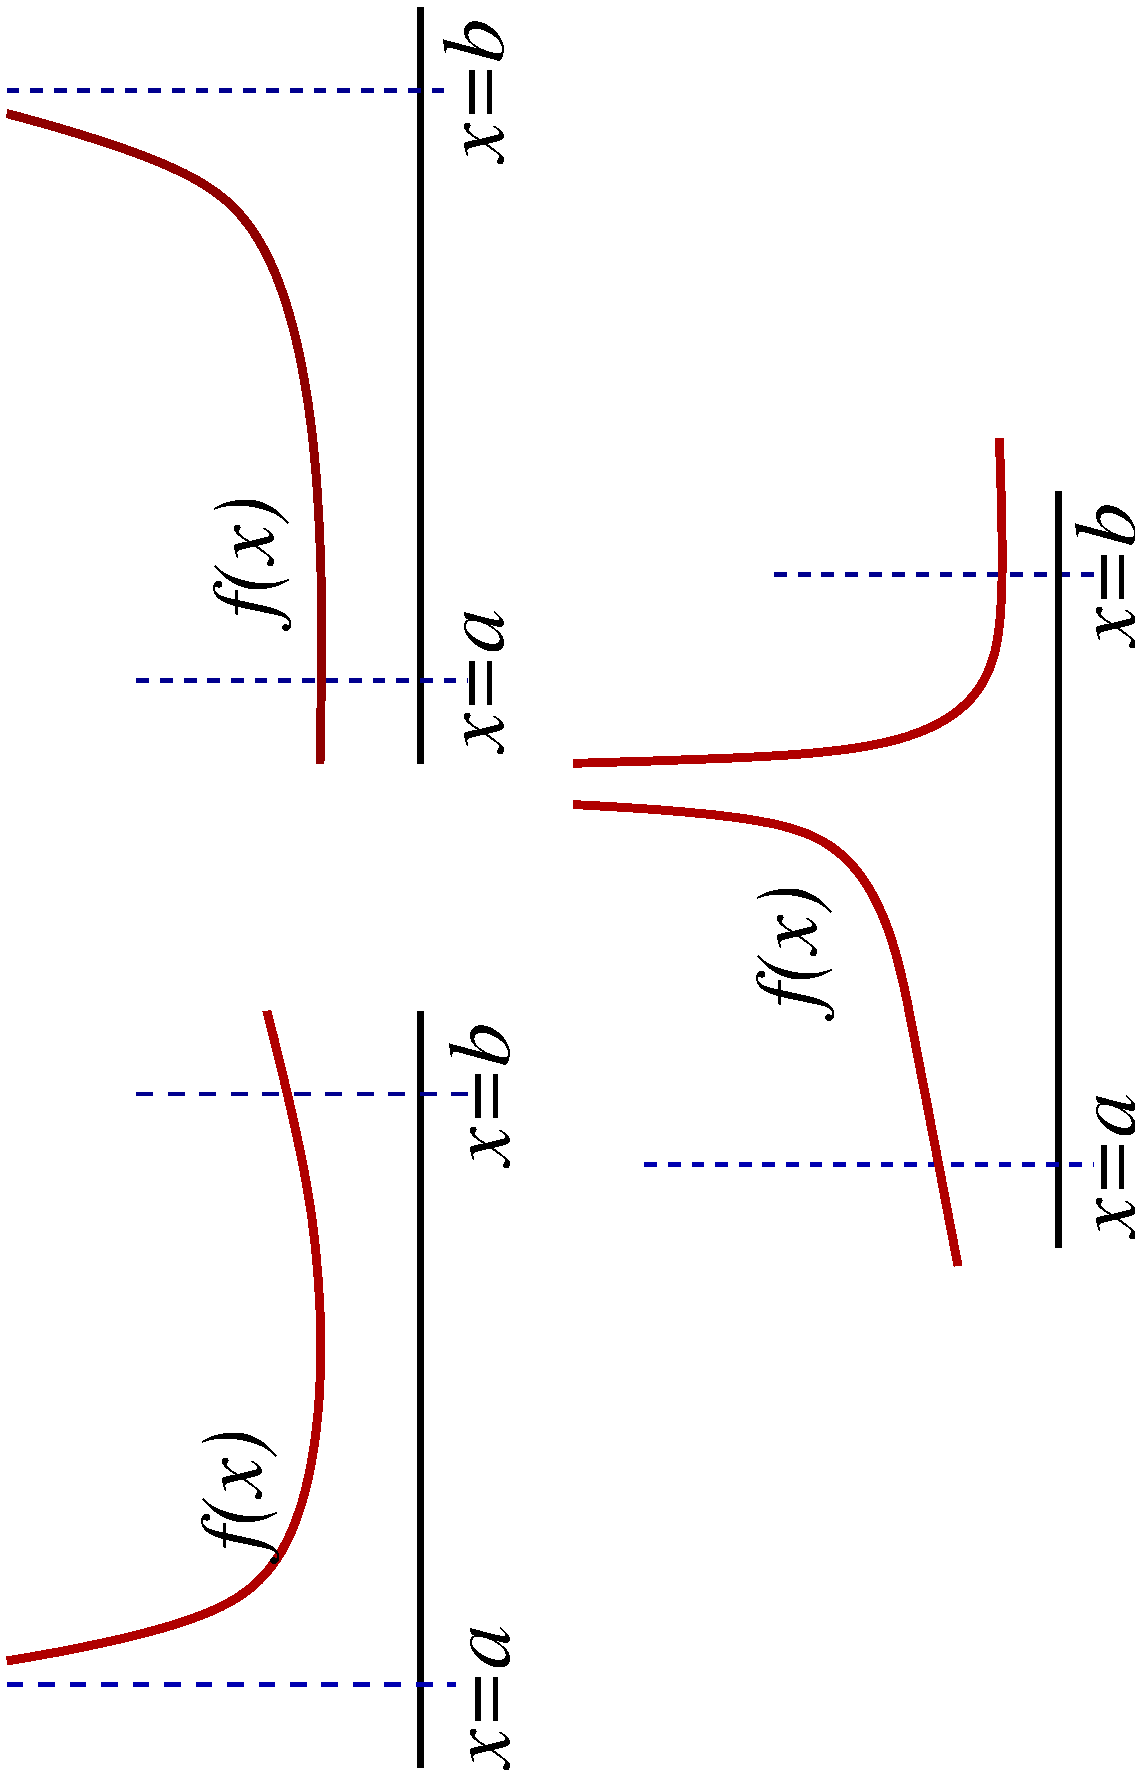
\includegraphics[width=4cm,angle=-90]{images/Improper2A}
\end{center}


% \end{columns}

}

\frame{
  \frametitle{Topics of the day...}

%\begin{columns}[c]
%\column{0.5\textwidth}
 \tableofcontents
%\column{0.5\textwidth}


See also Section 7.7 of Stewart.

%\end{columns}
}

\section{Proper Integrals}

\frame{

So far, the definite integrals we have considered:
\[  \int_a^b f(x) dx, \]
have all been \Emph{Proper}: they are integrals of bounded functions
on closed, finite intervals. 
\pause
\begin{columns}
\column{0.6\textwidth}
\begin{center}
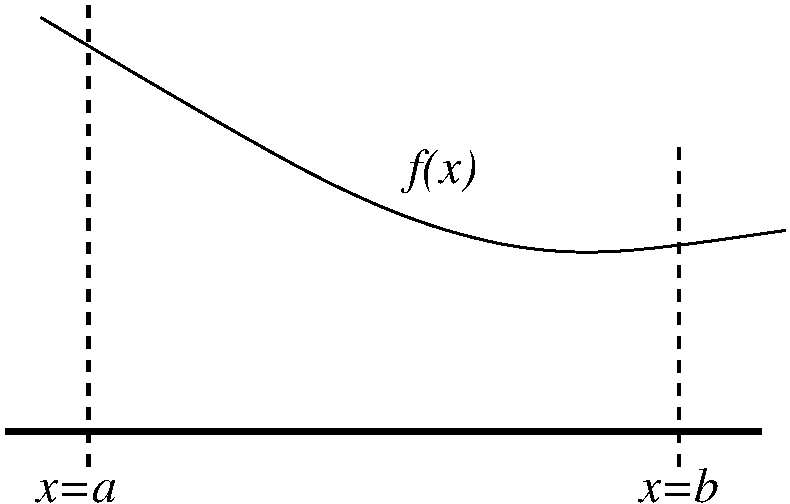
\includegraphics[width=6cm]{images/Proper}
\end{center}
\column{0.4\textwidth}
So we when we think of the integral as the area between the graph of
the function and the \eq{x}-axis, it is clear that that is
well-defined.
\end{columns}

}

\section{Improper Integrals}

\frame{
A definite integral \eqd{\int_a^b f(x) dx} is \Emph{Improper} if:


\begin{block}{\bf{Type I:} if $a = - \infty$ or $b= \infty$}
\begin{center}
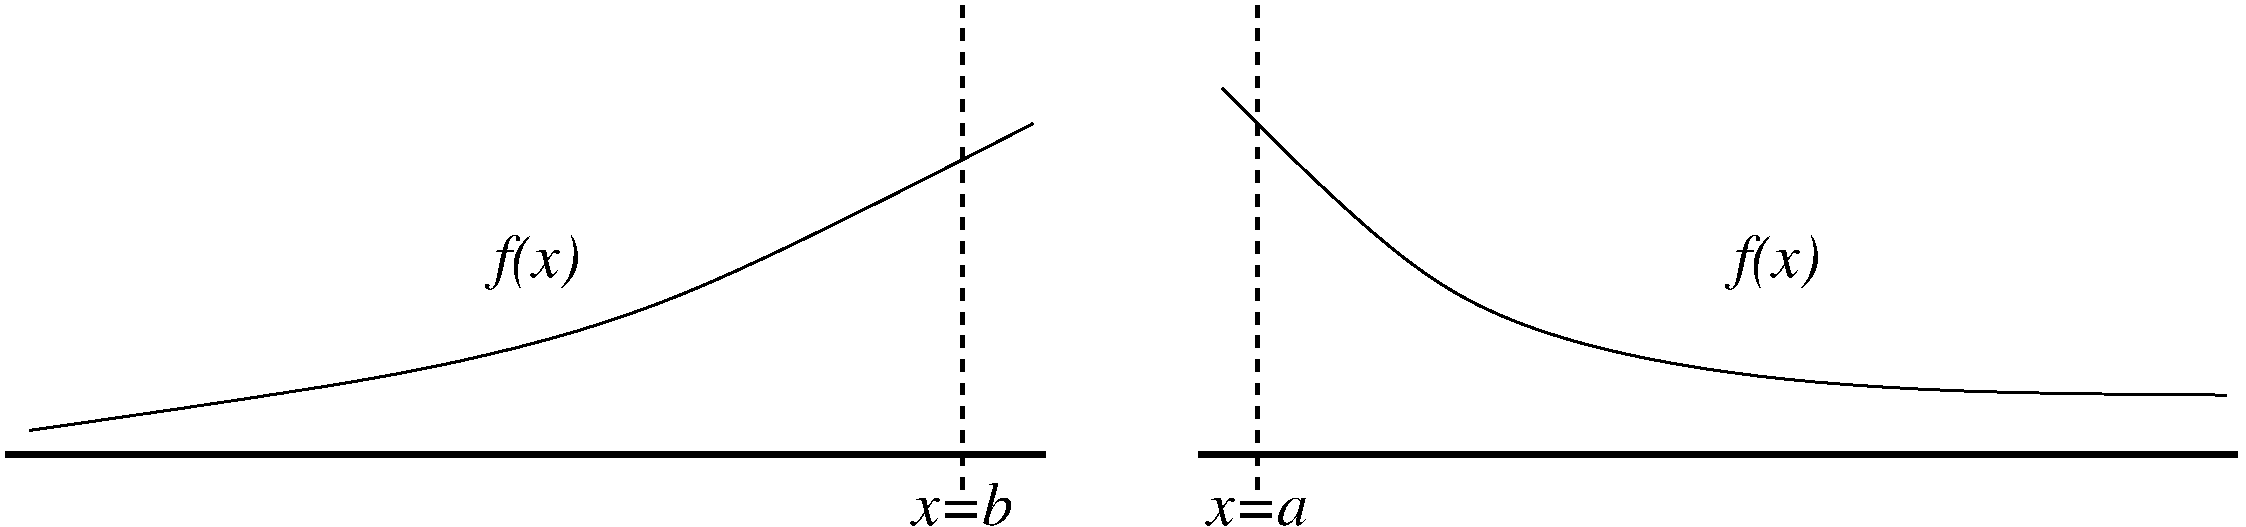
\includegraphics[width=9cm]{images/Improper1}
\end{center}
\end{block}


\begin{block}{\bf{Type II:} if $f(x)$  is unbounded (infinite) near $a$ or $b$.}
\begin{center}
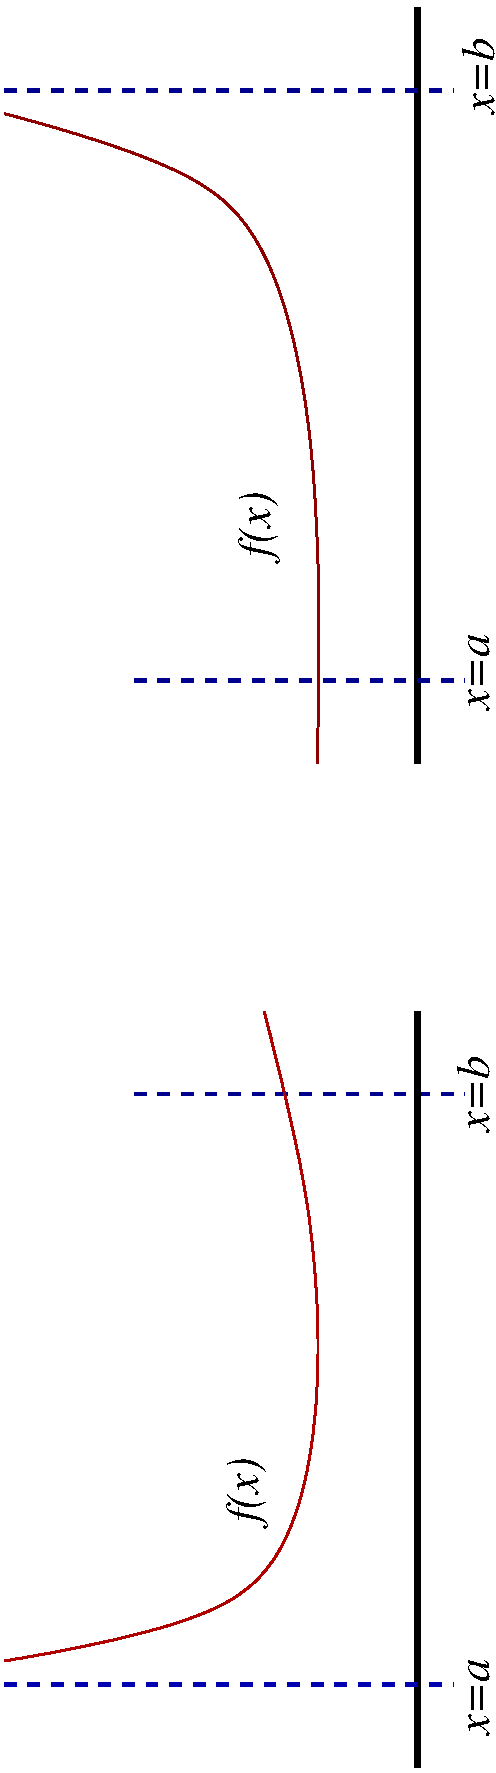
\includegraphics[width=2.4cm,angle=-90]{images/Improper2}
\end{center}
\end{block}


}

\frame{

\begin{itemize}
\item \Emph{Some} improper integrals evaluate as a real, finite
  number.  These are are said to \Bf{converge}, or to be
  \Emph{convergent} or \Bf{to exist}.  

\item Those that don't evaluate to a finite number are said to
  \Bf{diverge}, 
or to be \Emph{divergent} or \Bf{not to exist}.
\end{itemize}
}

\section{Improper Integrals of Type I} 
\frame{

\Bf{Improper Integrals of Type I } are of the form
\[ \int_{a}^{\infty} f(x)\,dx \quad  \text{ or } \quad
\int_{-\infty}^{b} f(x)\,dx.
\]
\begin{center}
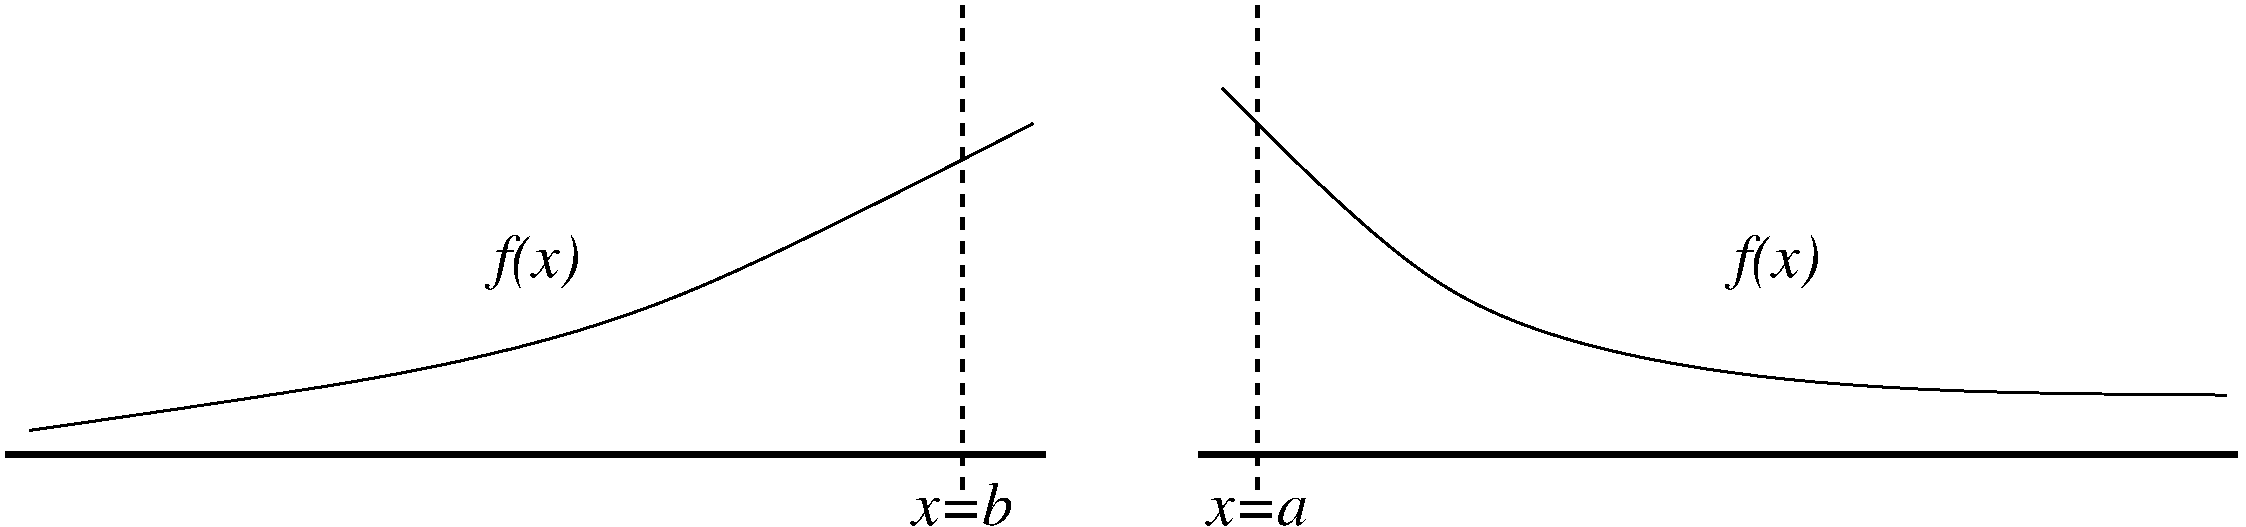
\includegraphics[width=9cm]{images/Improper1}
\end{center}

To evaluate these, note that \eqd{\int_a^\infty f(x) dx = \lim_{t = \infty}
\int_a^t f(x) dx}. So:
\begin{block}{}
\begin{itemize}
\item Evaluate \eqd{{\cal{I}}(t) = \int_a^t f(x) dx}; 
\item and then compute
\eqd{\lim_{t = \infty} \calI(t)}. 
\end{itemize}
\end{block}
}

%\section{Improper Integrals of Type I} 
\subsection{$\int_a^\infty f(x) dx$}


\frame{

\begin{columns}
\column{\textwidth-6cm}
\Header{~~~\eqd{\int_a^\infty f(x) dx}}
\column{6.5cm}
\begin{center}
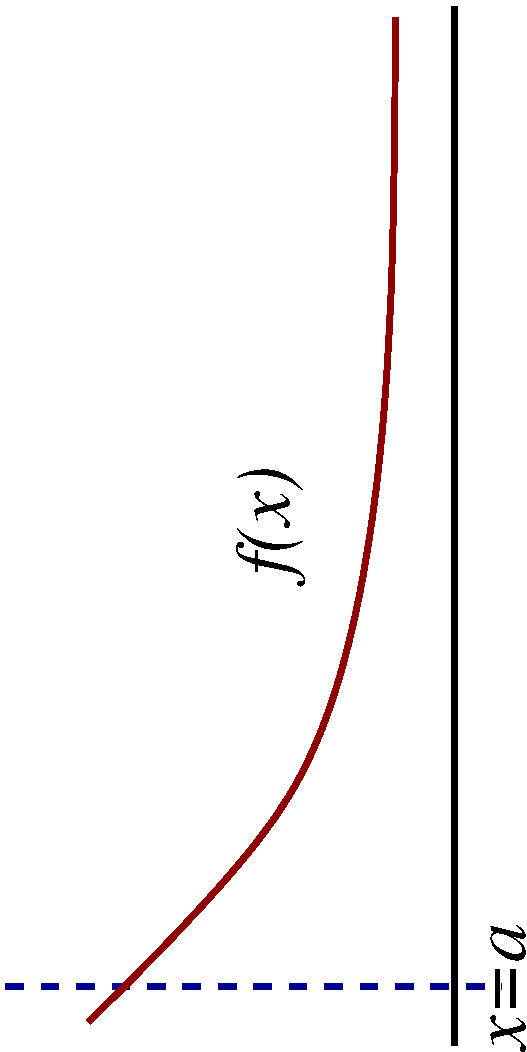
\includegraphics[angle=-90,width=6cm]{images/Improper1b}
\end{center}
\end{columns}
\begin{block}{}
\begin{enumerate}
\item Evaluate \eqd{{\cal{I}}(t) = \int_a^t f(x) dx}; 
\item and then compute
\eqd{\I = \lim_{t = \infty} \calI(t)}. 

\item If the limit  exists, call it $L$ and write $\int_{a}^{\infty} f(x)\,dx = L$.
We say that $\int_{a}^{\infty} f(x)\,dx$ {\bf converges to $L$}.

\item  If no such limit exists, $\int_{a}^{\infty} f(x)\,dx$ is said to {\bf diverge}.

\end{enumerate}
\end{block}
}

\frame{

\begin{example}
Evaluate \eqd{\I = \int_{1}^{\infty} \frac{1}{x^2}dx}
\end{example}
\vspace{4cm}
}

\frame{
\begin{example}
Evaluate the improper integral \eqd{\I = \int_{1}^{\infty} \frac{dx}{x}}
\end{example}
\vspace{4cm}
}

\frame{
\begin{example}
Evaluate \eqd{\I = \int_{1}^{\infty} \frac{1}{\sqrt{x}}dx}
\end{example}
\vspace{4cm}
}






\frame{
\begin{small}
\begin{block}{}%The general case}
\[ \int_{1}^{\infty} 1/x^{p}\,dx
\begin{cases} 
\texttt{\alert{converges}} & \text{for } p>1,\\
\texttt{\alert{diverges}} & \text{for}  p\leq 1.
\end{cases}
\]
\end{block}
\Bf{Proof:}
\pause
If  $p=1$ then\\  
\eqd{ ~~~  \int_1^t x^{-p} dx = \int_1^t \frac{1}{x} dx =
  \ln(x)\bigg|_1^t = \ln(t) - \ln(1) = \ln(t).}\\
But $\lim_{t\to\infty} \ln(t)$ does not exists,  so \eqd{\int_1^t \frac{1}{x} dx}
diverges.\\
\pause
If $p \neq 1$  then \eqd{\int_1^t x^{-p}dx = \frac{x^{1-p}}{1-p}\bigg|_1^t =
    \frac{t^{1-p} - 1}{1-p}}. \\
\pause If $p<1$ then $1-p>\alert{0}$ so the limit \eqd{\lim_{t\to\infty}  t^{1-p}}
does not exist,  so the integral diverges in that case.\\
\pause If however $p>1$ then $1-p<\alert{0}$ and  \eqd{\lim_{t\to\infty}  t^{1-p}=0},
so the integral converges to \eqd{\frac{-1}{1-p}}.
\end{small}
}


\frame{
\Header{Example: \eqd{\int_a^\infty x^{\alert{-2}} dx}}
\begin{center}
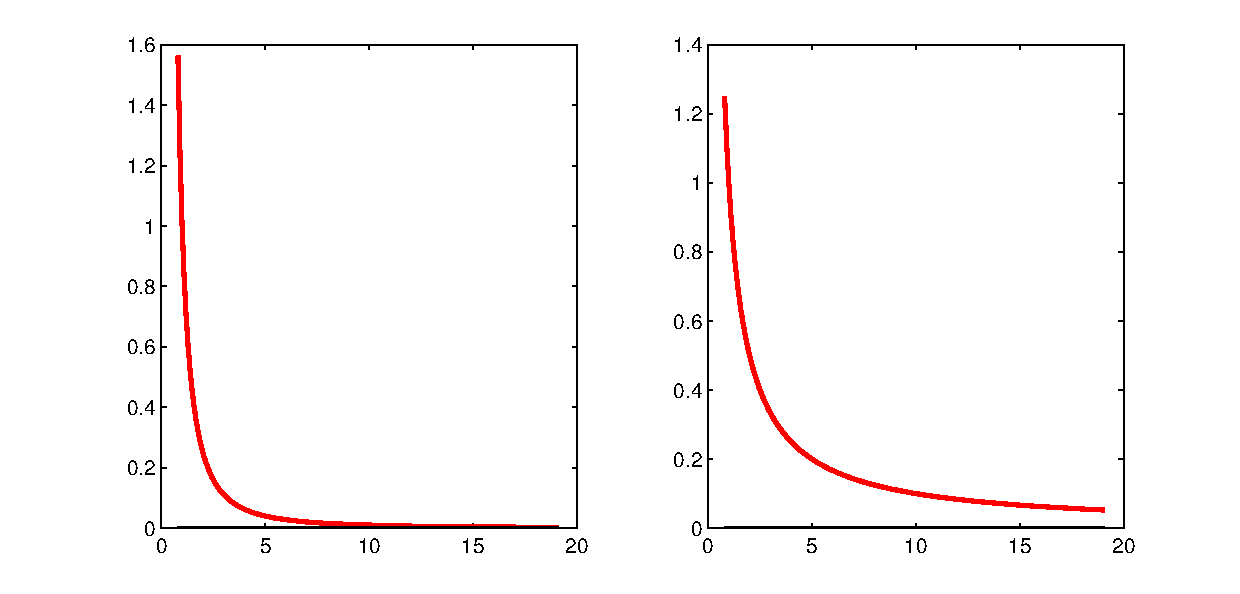
\includegraphics[width=12cm]{images/Impropx}
\end{center}
}
\frame{
\Header{Example: \eqd{\int_a^\infty x^{\alert{-1}} dx}}
\begin{center}
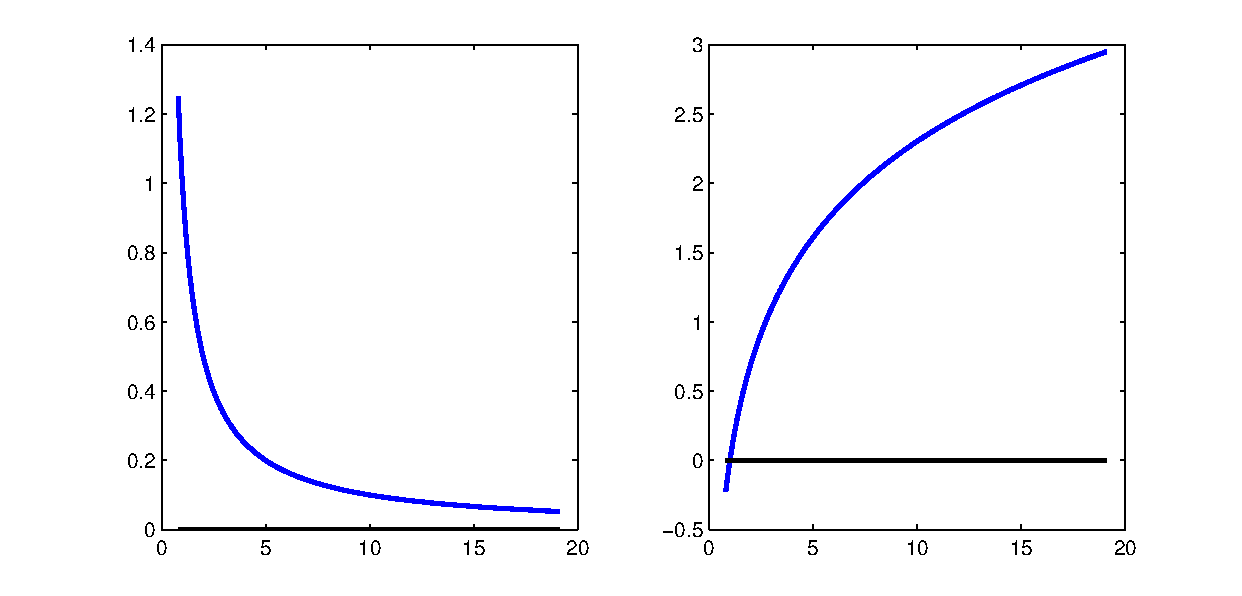
\includegraphics[width=12cm]{images/Improp_p=1.pdf}
\end{center}
}

\frame{
\Header{Example: \eqd{\int_a^\infty x^{\alert{-1/2}} dx}}
\begin{center}
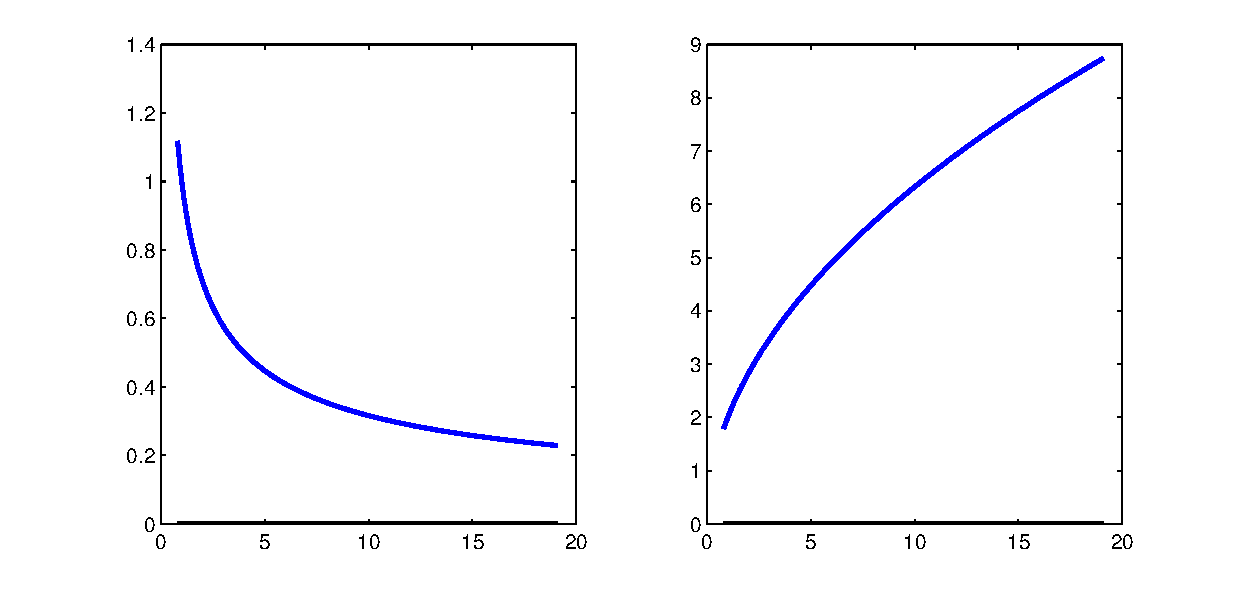
\includegraphics[width=12cm]{images/Improp_p_lt_1.pdf}
\end{center}
}


\frame{
\begin{example}
Evaluate the integral $\displaystyle\int_{1}^{\infty} \frac{1}{1+x^2}{dx}$
\end{example}
\vspace{4cm}
}



\subsection{$\int_{-\infty}^b f(x)dx$}

\frame{
\begin{columns}
\column{3cm}
For problems of the form:
\Header{\eqd{\int_{-\infty}^b f(x) dx}}
\column{6.5cm}
\begin{center}
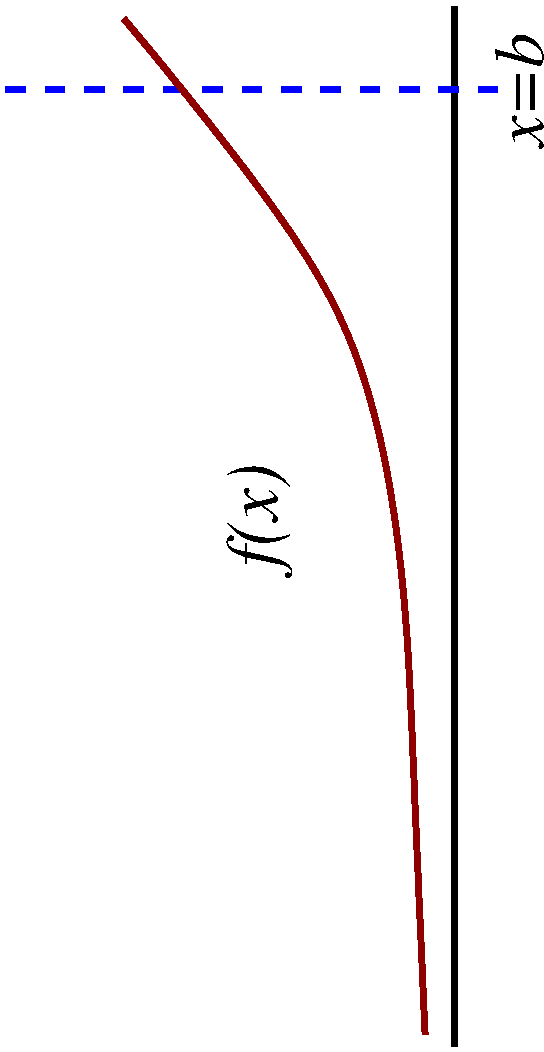
\includegraphics[angle=-90,width=6cm]{images/Improper1a}
\end{center}
\end{columns}

\begin{block}{}
\begin{enumerate}
\item Evaluate \eqd{{\cal{I}}(t) = \int_t^b f(x) dx}; 
\item and then compute
\eqd{\I = \lim_{t = -\infty} \calI(t)}. 

\item If the limit  exists, call it $\I$ and write $\int_{-\infty}^b f(x)\,dx = L$.
We say that the integral {\bf converges to $L$}.
\item  If no such limit
exists, it is said to {\bf diverge}.

\end{enumerate}
\end{block}
}



\frame{
\begin{example}
Evaluate $\displaystyle\int_{-\infty}^{-1} \frac{dx}{x^2}$
\end{example}
\vspace{4cm}
}

\frame{
\begin{example}
Show that  $\displaystyle\int_{-\infty}^{0} e^x dx$ converges, but that
$\displaystyle\int_{0}^{\infty} e^x dx$ diverges.

\end{example}
\vspace{4cm}
}

\subsection{$\int_{-\infty}^\infty f(x) dx$}
\frame{
We also have to deal with the case where \Emph{both} limits of
integration are at infinity:
\begin{columns}[c]
\column{0.3\textwidth}
\Header{ \eqd{\int_{-\infty}^{\infty} f(x)\,dx} }
\column{.6\textwidth}
\begin{center}
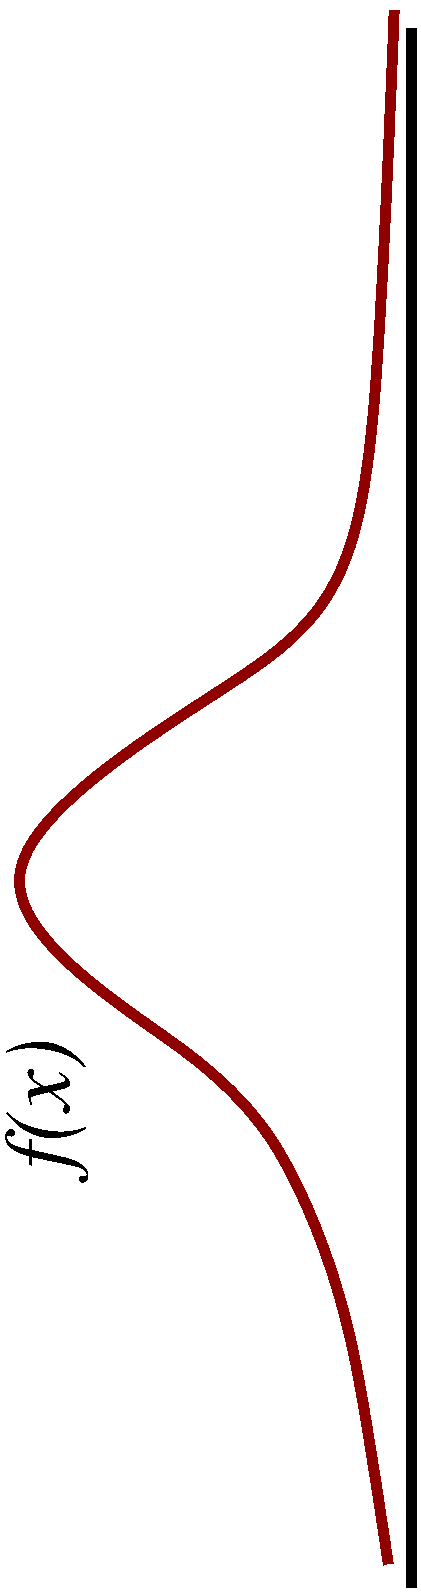
\includegraphics[angle=-90,width=6cm]{images/Improper1ab}
\end{center}
\end{columns}
To do this we recall that
\[
\int_{-\infty}^\infty f(x) dx = 
\int_{-\infty}^0 f(x) dx +
\int_0^\infty f(x) dx.
\]
So \eqd{\int_{-\infty}^\infty f(x) dx}  converge if and only if
\Emph{both} \eqd{\int_{-\infty}^{0} f(x)\,dx}  and
\eqd{\int_{0}^{\infty} f(x)\,dx} converge. 

}

\frame{
\begin{example}
Show that $\displaystyle\int_{-\infty}^{\infty} \frac{dx}{1 + x^2} =
\pi$
\end{example}
\vspace{4cm}

}


\frame{

\begin{exercise}[19.1]
Evaluate each of the following improper integrals:
\begin{enumerate}[(i)]
\item \eqd{\int_1^{\infty} \frac{1}{\ln(e^x)}dx}.
\hfill (ii) \eqd{\int_0^{\infty} \frac{x^2}{1+x^2}dx}.
\item[(iii)]  \eqd{\int_3^\infty \frac{dx}{(2x - 1)^{2/3}}}
\hfill (iv)  \eqd{\int_0^\infty \frac{x}{1 + 2x^2} dx}
\item[(v)] \eqd{\int_0^\infty \frac{1}{1 + e^x} dx}
\end{enumerate}
\end{exercise}
}

\end{document}

